\documentclass[a4paper,11pt]{article}
\usepackage[utf8]{inputenc}\usepackage[T1]{fontenc}
\usepackage[english]{babel}\usepackage{lmodern}\usepackage{microtype}
\usepackage{amsmath,amssymb}\usepackage{geometry}
\geometry{a4paper,left=2.2cm,right=2.2cm,top=2.0cm,bottom=2.0cm}
\usepackage{booktabs,array}\usepackage{xcolor}
\definecolor{bokug}{RGB}{0,135,60}\usepackage{tikz}
\usetikzlibrary{arrows.meta,calc}
\usepackage{fancyhdr}\pagestyle{fancy}
\renewcommand{\headrulewidth}{0.4pt}
\usepackage{enumitem}\setlength{\parindent}{0pt}\setlength{\parskip}{4pt}

\begin{document}
\fancyhead[L]{\small VU Mechanik – LAWI 100515 (PI)}\fancyhead[R]{\small SS 2026}\fancyfoot[C]{\thepage}
\begin{center}{\large\bfseries\color{bokug}University of Natural Resources and Life Sciences, Vienna (BOKU)}\\[2pt]{\large\bfseries VU Mechanik – LAWI 100515 (PI)}\\[4pt]Exam \textbf{Group A} \hfill Date: 26.06.2026\\[2pt]\rule{\linewidth}{0.4pt}\end{center}

\begin{center}\textbf{\large Model solution}\end{center}
\begin{center}
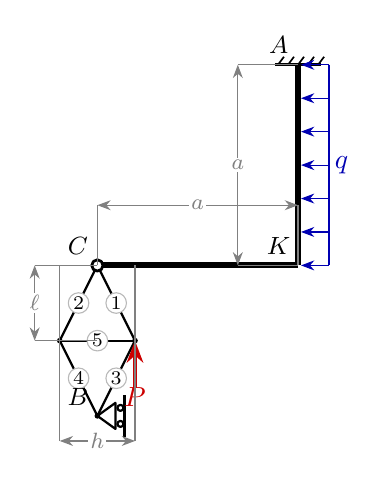
\begin{tikzpicture}[scale=0.637,>=Stealth,line join=round]
  \coordinate (P0) at (0.000,0.000);
  \coordinate (K) at (0.000,-4.000);
  \coordinate (C) at (-4.000,-4.000);
  \coordinate (TO1) at (-3.250,-5.500);
  \coordinate (TU0) at (-4.750,-5.500);
  \coordinate (TO2) at (-4.000,-7.000);
  \draw[thick] (C) -- (TO1);
  \draw[thick] (C) -- (TU0);
  \draw[thick] (TO1) -- (TO2);
  \draw[thick] (TU0) -- (TO2);
  \draw[thick] (TO1) -- (TU0);
  \draw[line width=2.2pt] (P0) -- (K);
  \draw[line width=2.2pt] (K) -- (C);
  \fill (TO1) circle (1.6pt);
  \fill (TU0) circle (1.6pt);
  \fill (TO2) circle (1.6pt);
  \draw[fill=white,line width=1pt] (C) circle (3.2pt);
  \draw[line width=1.1pt] (0.450,0.000) -- (-0.450,0.000);
  \draw[line width=0.6pt] (0.400,0.000) -- (0.520,0.160);
  \draw[line width=0.6pt] (0.200,0.000) -- (0.320,0.160);
  \draw[line width=0.6pt] (0.000,0.000) -- (0.120,0.160);
  \draw[line width=0.6pt] (-0.200,0.000) -- (-0.080,0.160);
  \draw[line width=0.6pt] (-0.400,0.000) -- (-0.280,0.160);
  \draw[thick] (-4.000,-7.000) -- (-3.640,-7.260) -- (-3.640,-6.740) -- cycle;
  \draw[thick] (-3.540,-7.160) circle (0.06) (-3.540,-6.840) circle (0.06);
  \draw[line width=1pt] (-3.460,-7.420) -- (-3.460,-6.580);
  \node[circle,fill=white,draw=gray!55,inner sep=0.5pt,font=\scriptsize] at (-3.625,-4.750) {1};
  \node[circle,fill=white,draw=gray!55,inner sep=0.5pt,font=\scriptsize] at (-4.375,-4.750) {2};
  \node[circle,fill=white,draw=gray!55,inner sep=0.5pt,font=\scriptsize] at (-3.625,-6.250) {3};
  \node[circle,fill=white,draw=gray!55,inner sep=0.5pt,font=\scriptsize] at (-4.375,-6.250) {4};
  \node[circle,fill=white,draw=gray!55,inner sep=0.5pt,font=\scriptsize] at (-4.000,-5.500) {5};
  \draw[->,blue!70!black] (0.620,0.000) -- (0.060,0.000);
  \draw[->,blue!70!black] (0.620,-0.667) -- (0.060,-0.667);
  \draw[->,blue!70!black] (0.620,-1.333) -- (0.060,-1.333);
  \draw[->,blue!70!black] (0.620,-2.000) -- (0.060,-2.000);
  \draw[->,blue!70!black] (0.620,-2.667) -- (0.060,-2.667);
  \draw[->,blue!70!black] (0.620,-3.333) -- (0.060,-3.333);
  \draw[->,blue!70!black] (0.620,-4.000) -- (0.060,-4.000);
  \draw[blue!70!black,thick] (0.620,0.000) -- (0.620,-4.000);
  \node[blue!70!black] at (0.870,-2.000) {$q$};
  \draw[->,red!80!black,line width=1.1pt] (-3.250,-6.450) -- (-3.250,-5.500);
  \node[red!80!black] at (-3.250,-6.630) {$P$};
  \draw[thin,gray] (0.000,0.000) -- (-1.200,0.000);
  \draw[thin,gray] (0.000,-4.000) -- (-1.200,-4.000);
  \draw[<->,gray] (-1.200,0.000) -- (-1.200,-4.000) node[midway,fill=white,inner sep=0.8pt,font=\footnotesize]{$a$};
  \draw[thin,gray] (0.000,-4.000) -- (0.000,-2.800);
  \draw[thin,gray] (-4.000,-4.000) -- (-4.000,-2.800);
  \draw[<->,gray] (0.000,-2.800) -- (-4.000,-2.800) node[midway,fill=white,inner sep=0.8pt,font=\footnotesize]{$a$};
  \draw[thin,gray] (-4.000,-4.000) -- (-5.250,-4.000);
  \draw[thin,gray] (-4.000,-5.500) -- (-5.250,-5.500);
  \draw[<->,gray] (-5.250,-4.000) -- (-5.250,-5.500) node[midway,fill=white,inner sep=0.8pt,font=\footnotesize]{$\ell$};
  \draw[thin,gray] (-3.250,-4.000) -- (-3.250,-7.500);
  \draw[thin,gray] (-4.750,-4.000) -- (-4.750,-7.500);
  \draw[<->,gray] (-3.250,-7.500) -- (-4.750,-7.500) node[midway,fill=white,inner sep=0.8pt,font=\footnotesize]{$h$};
  \node[font=\small] at (0.000,0.000) [xshift=-7pt,yshift=7pt] {$A$};
  \node[font=\small] at (0.000,-4.000) [xshift=-7pt,yshift=7pt] {$K$};
  \node[font=\small] at (-4.000,-4.000) [xshift=-7pt,yshift=7pt] {$C$};
  \node[font=\small] at (-4.000,-7.000) [xshift=-7pt,yshift=7pt] {$B$};
\end{tikzpicture}
\end{center}
\par\medskip\textbf{1.\ Static determinacy}\par Counting criterion $n=3k-(a+z)$ (bodies $k$, reactions $a$, interaction forces $z$):
\[ n=3k-(a+z)=3\cdot2-(4+2)=0\ \Rightarrow\ \text{statically determinate} \]
\par\medskip\textbf{2.\ Support reactions and hinge forces}\par
$A:\ R_x=19,\ R_y=-12,\ M=92$\quad $B:\ R_x=-3,\ R_y=0$\par $C:\ H_x=-3,\ H_y=12$
\par\medskip\textbf{3.\ Truss member forces}\par
\begin{center}\renewcommand{\arraystretch}{1.1}\begin{tabular}{c r l}
\toprule
Member & Force $S$ [kN] & Type \\
\midrule
  1 & -10.06 & compression \\
  2 & -3.35 & compression \\
  3 & 3.35 & tension \\
  4 & -3.35 & compression \\
  5 & 3 & tension \\
\bottomrule
\end{tabular}\end{center}
\begin{center}
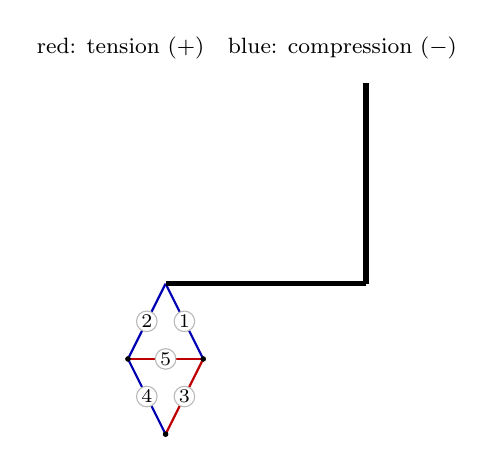
\begin{tikzpicture}[scale=0.637,>=Stealth,line join=round]
  \coordinate (P0) at (0.000,0.000);
  \coordinate (K) at (0.000,-4.000);
  \coordinate (C) at (-4.000,-4.000);
  \coordinate (TO1) at (-3.250,-5.500);
  \coordinate (TU0) at (-4.750,-5.500);
  \coordinate (TO2) at (-4.000,-7.000);
  \draw[thick,blue!70!black] (C) -- (TO1);
  \draw[thick,blue!70!black] (C) -- (TU0);
  \draw[thick,red!75!black] (TO1) -- (TO2);
  \draw[thick,blue!70!black] (TU0) -- (TO2);
  \draw[thick,red!75!black] (TO1) -- (TU0);
  \draw[line width=2pt] (P0) -- (K);
  \draw[line width=2pt] (K) -- (C);
  \fill (TO1) circle (1.6pt);
  \fill (TU0) circle (1.6pt);
  \fill (TO2) circle (1.6pt);
  \node[circle,fill=white,draw=gray!55,inner sep=0.5pt,font=\scriptsize] at (-3.625,-4.750) {1};
  \node[circle,fill=white,draw=gray!55,inner sep=0.5pt,font=\scriptsize] at (-4.375,-4.750) {2};
  \node[circle,fill=white,draw=gray!55,inner sep=0.5pt,font=\scriptsize] at (-3.625,-6.250) {3};
  \node[circle,fill=white,draw=gray!55,inner sep=0.5pt,font=\scriptsize] at (-4.375,-6.250) {4};
  \node[circle,fill=white,draw=gray!55,inner sep=0.5pt,font=\scriptsize] at (-4.000,-5.500) {5};
  \node[font=\footnotesize] at (-2.38,0.70) {red: tension $(+)$\quad blue: compression $(-)$};
\end{tikzpicture}
\end{center}
\par\medskip\textbf{4.\ Section-force diagrams of the beams}\par
\begin{center}
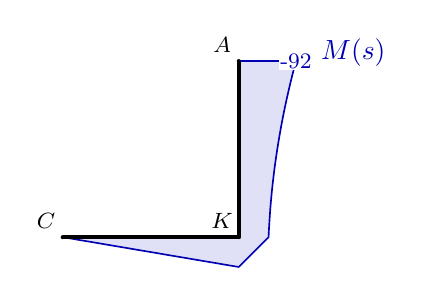
\begin{tikzpicture}[scale=0.559,line join=round]
  \filldraw[fill=blue!70!black!12,draw=blue!70!black,semithick] (1.300,0.000) -- (1.256,-0.167) -- (1.214,-0.333) -- (1.173,-0.500) -- (1.134,-0.667) -- (1.096,-0.833) -- (1.060,-1.000) -- (1.025,-1.167) -- (0.992,-1.333) -- (0.961,-1.500) -- (0.931,-1.667) -- (0.903,-1.833) -- (0.876,-2.000) -- (0.851,-2.167) -- (0.827,-2.333) -- (0.805,-2.500) -- (0.785,-2.667) -- (0.766,-2.833) -- (0.749,-3.000) -- (0.733,-3.167) -- (0.719,-3.333) -- (0.707,-3.500) -- (0.696,-3.667) -- (0.686,-3.833) -- (0.678,-4.000) -- (0.000,-4.678) -- (-0.167,-4.650) -- (-0.333,-4.622) -- (-0.500,-4.593) -- (-0.667,-4.565) -- (-0.833,-4.537) -- (-1.000,-4.509) -- (-1.167,-4.480) -- (-1.333,-4.452) -- (-1.500,-4.424) -- (-1.667,-4.396) -- (-1.833,-4.367) -- (-2.000,-4.339) -- (-2.167,-4.311) -- (-2.333,-4.283) -- (-2.500,-4.254) -- (-2.667,-4.226) -- (-2.833,-4.198) -- (-3.000,-4.170) -- (-3.167,-4.141) -- (-3.333,-4.113) -- (-3.500,-4.085) -- (-3.667,-4.057) -- (-3.833,-4.028) -- (-4.000,-4.000) -- (-4.000,-4.000) -- (-3.833,-4.000) -- (-3.667,-4.000) -- (-3.500,-4.000) -- (-3.333,-4.000) -- (-3.167,-4.000) -- (-3.000,-4.000) -- (-2.833,-4.000) -- (-2.667,-4.000) -- (-2.500,-4.000) -- (-2.333,-4.000) -- (-2.167,-4.000) -- (-2.000,-4.000) -- (-1.833,-4.000) -- (-1.667,-4.000) -- (-1.500,-4.000) -- (-1.333,-4.000) -- (-1.167,-4.000) -- (-1.000,-4.000) -- (-0.833,-4.000) -- (-0.667,-4.000) -- (-0.500,-4.000) -- (-0.333,-4.000) -- (-0.167,-4.000) -- (0.000,-4.000) -- (0.000,-4.000) -- (0.000,-3.833) -- (0.000,-3.667) -- (0.000,-3.500) -- (0.000,-3.333) -- (0.000,-3.167) -- (0.000,-3.000) -- (0.000,-2.833) -- (0.000,-2.667) -- (0.000,-2.500) -- (0.000,-2.333) -- (0.000,-2.167) -- (0.000,-2.000) -- (0.000,-1.833) -- (0.000,-1.667) -- (0.000,-1.500) -- (0.000,-1.333) -- (0.000,-1.167) -- (0.000,-1.000) -- (0.000,-0.833) -- (0.000,-0.667) -- (0.000,-0.500) -- (0.000,-0.333) -- (0.000,-0.167) -- (0.000,0.000) -- cycle;
  \draw[line width=1.6pt] (0.000,0.000) -- (0.000,-4.000) -- (-4.000,-4.000);
  \node[blue!70!black,font=\footnotesize,fill=white,inner sep=0.5pt] at (1.300,0.000) {-92};
  \fill (0.000,0.000) circle (1.3pt);
  \node[font=\footnotesize] at (0.000,0.000) [xshift=-6pt,yshift=6pt] {$A$};
  \fill (0.000,-4.000) circle (1.3pt);
  \node[font=\footnotesize] at (0.000,-4.000) [xshift=-6pt,yshift=6pt] {$K$};
  \fill (-4.000,-4.000) circle (1.3pt);
  \node[font=\footnotesize] at (-4.000,-4.000) [xshift=-6pt,yshift=6pt] {$C$};
  \node[blue!70!black,right] at (1.65,0.20) {$M(s)$};
\end{tikzpicture}\\[5pt]
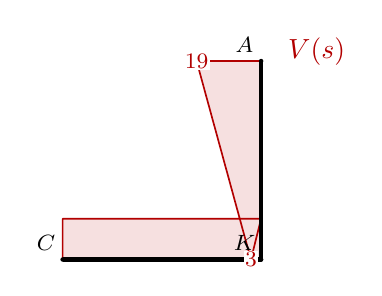
\begin{tikzpicture}[scale=0.630,line join=round]
  \filldraw[fill=red!70!black!12,draw=red!70!black,semithick] (-1.300,0.000) -- (-1.254,-0.167) -- (-1.209,-0.333) -- (-1.163,-0.500) -- (-1.118,-0.667) -- (-1.072,-0.833) -- (-1.026,-1.000) -- (-0.981,-1.167) -- (-0.935,-1.333) -- (-0.889,-1.500) -- (-0.844,-1.667) -- (-0.798,-1.833) -- (-0.753,-2.000) -- (-0.707,-2.167) -- (-0.661,-2.333) -- (-0.616,-2.500) -- (-0.570,-2.667) -- (-0.525,-2.833) -- (-0.479,-3.000) -- (-0.433,-3.167) -- (-0.388,-3.333) -- (-0.342,-3.500) -- (-0.296,-3.667) -- (-0.251,-3.833) -- (-0.205,-4.000) -- (0.000,-3.179) -- (-0.167,-3.179) -- (-0.333,-3.179) -- (-0.500,-3.179) -- (-0.667,-3.179) -- (-0.833,-3.179) -- (-1.000,-3.179) -- (-1.167,-3.179) -- (-1.333,-3.179) -- (-1.500,-3.179) -- (-1.667,-3.179) -- (-1.833,-3.179) -- (-2.000,-3.179) -- (-2.167,-3.179) -- (-2.333,-3.179) -- (-2.500,-3.179) -- (-2.667,-3.179) -- (-2.833,-3.179) -- (-3.000,-3.179) -- (-3.167,-3.179) -- (-3.333,-3.179) -- (-3.500,-3.179) -- (-3.667,-3.179) -- (-3.833,-3.179) -- (-4.000,-3.179) -- (-4.000,-4.000) -- (-3.833,-4.000) -- (-3.667,-4.000) -- (-3.500,-4.000) -- (-3.333,-4.000) -- (-3.167,-4.000) -- (-3.000,-4.000) -- (-2.833,-4.000) -- (-2.667,-4.000) -- (-2.500,-4.000) -- (-2.333,-4.000) -- (-2.167,-4.000) -- (-2.000,-4.000) -- (-1.833,-4.000) -- (-1.667,-4.000) -- (-1.500,-4.000) -- (-1.333,-4.000) -- (-1.167,-4.000) -- (-1.000,-4.000) -- (-0.833,-4.000) -- (-0.667,-4.000) -- (-0.500,-4.000) -- (-0.333,-4.000) -- (-0.167,-4.000) -- (0.000,-4.000) -- (0.000,-4.000) -- (0.000,-3.833) -- (0.000,-3.667) -- (0.000,-3.500) -- (0.000,-3.333) -- (0.000,-3.167) -- (0.000,-3.000) -- (0.000,-2.833) -- (0.000,-2.667) -- (0.000,-2.500) -- (0.000,-2.333) -- (0.000,-2.167) -- (0.000,-2.000) -- (0.000,-1.833) -- (0.000,-1.667) -- (0.000,-1.500) -- (0.000,-1.333) -- (0.000,-1.167) -- (0.000,-1.000) -- (0.000,-0.833) -- (0.000,-0.667) -- (0.000,-0.500) -- (0.000,-0.333) -- (0.000,-0.167) -- (0.000,0.000) -- cycle;
  \draw[line width=1.6pt] (0.000,0.000) -- (0.000,-4.000) -- (-4.000,-4.000);
  \node[red!70!black,font=\footnotesize,fill=white,inner sep=0.5pt] at (-1.300,0.000) {19};
  \node[red!70!black,font=\footnotesize,fill=white,inner sep=0.5pt] at (-0.205,-4.000) {3};
  \fill (0.000,0.000) circle (1.3pt);
  \node[font=\footnotesize] at (0.000,0.000) [xshift=-6pt,yshift=6pt] {$A$};
  \fill (0.000,-4.000) circle (1.3pt);
  \node[font=\footnotesize] at (0.000,-4.000) [xshift=-6pt,yshift=6pt] {$K$};
  \fill (-4.000,-4.000) circle (1.3pt);
  \node[font=\footnotesize] at (-4.000,-4.000) [xshift=-6pt,yshift=6pt] {$C$};
  \node[red!70!black,right] at (0.35,0.20) {$V(s)$};
\end{tikzpicture}\\[5pt]
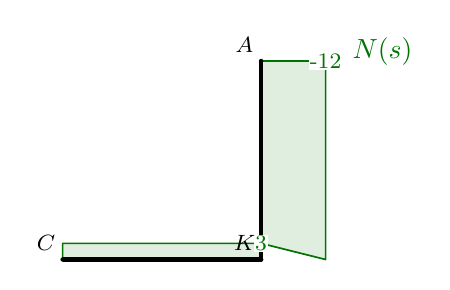
\begin{tikzpicture}[scale=0.630,line join=round]
  \filldraw[fill=green!45!black!12,draw=green!45!black,semithick] (1.300,0.000) -- (1.300,-0.167) -- (1.300,-0.333) -- (1.300,-0.500) -- (1.300,-0.667) -- (1.300,-0.833) -- (1.300,-1.000) -- (1.300,-1.167) -- (1.300,-1.333) -- (1.300,-1.500) -- (1.300,-1.667) -- (1.300,-1.833) -- (1.300,-2.000) -- (1.300,-2.167) -- (1.300,-2.333) -- (1.300,-2.500) -- (1.300,-2.667) -- (1.300,-2.833) -- (1.300,-3.000) -- (1.300,-3.167) -- (1.300,-3.333) -- (1.300,-3.500) -- (1.300,-3.667) -- (1.300,-3.833) -- (1.300,-4.000) -- (0.000,-3.675) -- (-0.167,-3.675) -- (-0.333,-3.675) -- (-0.500,-3.675) -- (-0.667,-3.675) -- (-0.833,-3.675) -- (-1.000,-3.675) -- (-1.167,-3.675) -- (-1.333,-3.675) -- (-1.500,-3.675) -- (-1.667,-3.675) -- (-1.833,-3.675) -- (-2.000,-3.675) -- (-2.167,-3.675) -- (-2.333,-3.675) -- (-2.500,-3.675) -- (-2.667,-3.675) -- (-2.833,-3.675) -- (-3.000,-3.675) -- (-3.167,-3.675) -- (-3.333,-3.675) -- (-3.500,-3.675) -- (-3.667,-3.675) -- (-3.833,-3.675) -- (-4.000,-3.675) -- (-4.000,-4.000) -- (-3.833,-4.000) -- (-3.667,-4.000) -- (-3.500,-4.000) -- (-3.333,-4.000) -- (-3.167,-4.000) -- (-3.000,-4.000) -- (-2.833,-4.000) -- (-2.667,-4.000) -- (-2.500,-4.000) -- (-2.333,-4.000) -- (-2.167,-4.000) -- (-2.000,-4.000) -- (-1.833,-4.000) -- (-1.667,-4.000) -- (-1.500,-4.000) -- (-1.333,-4.000) -- (-1.167,-4.000) -- (-1.000,-4.000) -- (-0.833,-4.000) -- (-0.667,-4.000) -- (-0.500,-4.000) -- (-0.333,-4.000) -- (-0.167,-4.000) -- (0.000,-4.000) -- (0.000,-4.000) -- (0.000,-3.833) -- (0.000,-3.667) -- (0.000,-3.500) -- (0.000,-3.333) -- (0.000,-3.167) -- (0.000,-3.000) -- (0.000,-2.833) -- (0.000,-2.667) -- (0.000,-2.500) -- (0.000,-2.333) -- (0.000,-2.167) -- (0.000,-2.000) -- (0.000,-1.833) -- (0.000,-1.667) -- (0.000,-1.500) -- (0.000,-1.333) -- (0.000,-1.167) -- (0.000,-1.000) -- (0.000,-0.833) -- (0.000,-0.667) -- (0.000,-0.500) -- (0.000,-0.333) -- (0.000,-0.167) -- (0.000,0.000) -- cycle;
  \draw[line width=1.6pt] (0.000,0.000) -- (0.000,-4.000) -- (-4.000,-4.000);
  \node[green!45!black,font=\footnotesize,fill=white,inner sep=0.5pt] at (1.300,0.000) {-12};
  \node[green!45!black,font=\footnotesize,fill=white,inner sep=0.5pt] at (0.000,-3.675) {3};
  \fill (0.000,0.000) circle (1.3pt);
  \node[font=\footnotesize] at (0.000,0.000) [xshift=-6pt,yshift=6pt] {$A$};
  \fill (0.000,-4.000) circle (1.3pt);
  \node[font=\footnotesize] at (0.000,-4.000) [xshift=-6pt,yshift=6pt] {$K$};
  \fill (-4.000,-4.000) circle (1.3pt);
  \node[font=\footnotesize] at (-4.000,-4.000) [xshift=-6pt,yshift=6pt] {$C$};
  \node[green!45!black,right] at (1.65,0.20) {$N(s)$};
\end{tikzpicture}\\[10pt]
\end{center}
\end{document}